%!TeX root =  ../../thesis.tex

\subsection{Raspberry Pi}
Raspberry Pi je značka jednodeskových počítačů na kterých je primárně operační systém Raspberry Pi OS (dříve Raspbian). Jedná se odlehčenou linuxovou distribuci, která je založena na linuxové distribuci Debian, které je známá svou stabilitou. Raspberry Pi je původem ze Spojeného Království a je vhodné pro začátečníky v IoT, jelikož použití je intuitivnější a také se na něm dá vyvíjet pomocí Pythonu.
\begin{figure}[H]
	\centering
	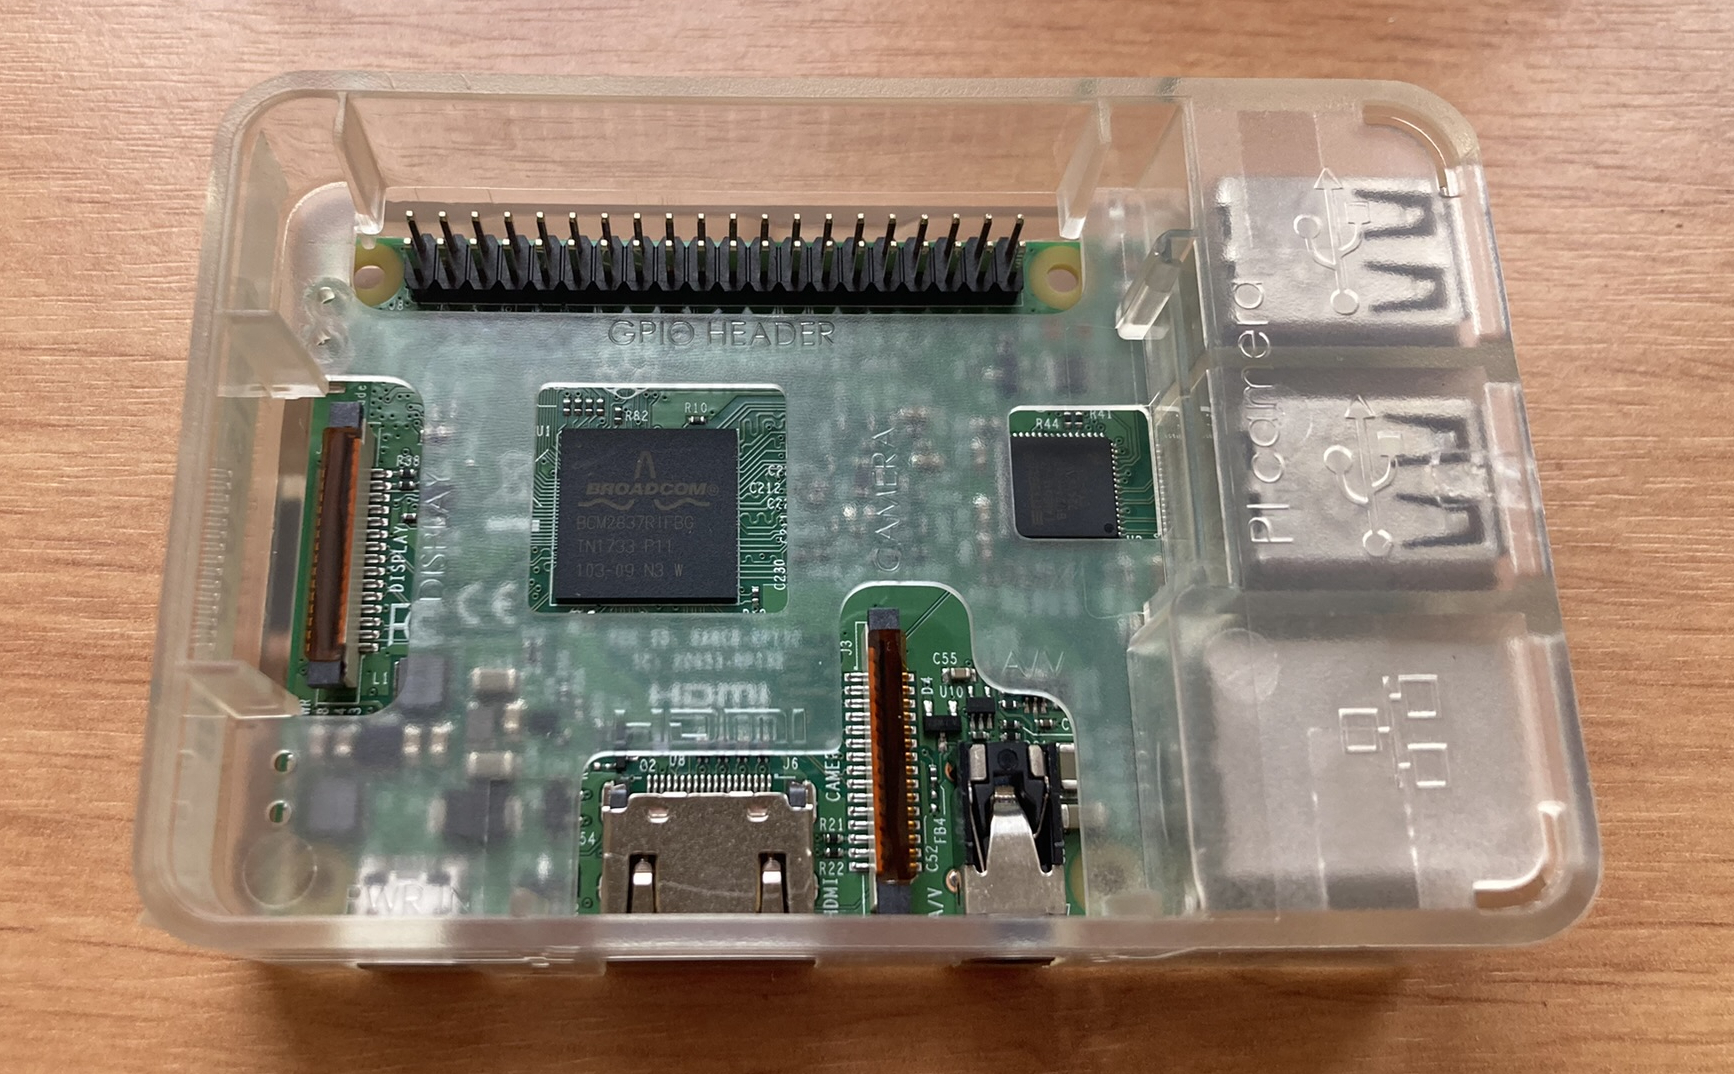
\includegraphics[width=0.9\textwidth]{pictures/rasp.jpeg}
    	\caption{Raspberry Pi}
   	\label{fig:rasPI}
\end{figure}
Na obrázku \ref{fig:rasPI} vidíme Rapsberry PI, které je v plastovém obalu s výřezy pro přístup na IO, včetně pinového headeru, na který se dá připojit shield s polem led žároviček. Také vidíme USB a RJ-45 konektor a další konektory, ovšem já se momentálně nevěnuji práci s Rapsberry Pi, tudíž mu v této bakalářské práci nebudu věnovat tolik pozornosti, nicméně jej bylo důležité zmínit, jelikož patří mezi významné jednodeskové počítače.